\documentclass[a4paper, 12pt]{report}

%%%%%%%%%%%%
% Packages %
%%%%%%%%%%%%

\usepackage[english]{babel}
\usepackage[noheader]{packages/sleek}
\usepackage{packages/sleek-title}
\usepackage{packages/sleek-theorems}
\usepackage{packages/sleek-listings}
\usepackage{wrapfig}

\graphicspath{ {./resources/img/} }

%%%%%%%%%%%%%%
% Title-page %
%%%%%%%%%%%%%%

\logo{./resources/img/IIT-Madras-01.eps}
\institute{Indian Institute of Technology Madras}
\faculty{Computer Science and Engineering Department}
\department{\textsc{Faculty:} Prof. Balaraman Ravindran}
\title{Lecture Notes on:}
\subtitle{Introduction to Reinforcement Learning}
\author{\textit{Author}\\Jashaswimalya \textsc{Acharjee}}
\supervisor{\textit{Instructor}\\Prof. Balaraman \textsc{Ravindran}}
\context{To summarise my experience in the class of\\\texttt{CS6700: Intro to Reinforcement Learning}}
\date{Jan-May, 2023}

%%%%%%%%%%%%%%%%
% Bibliography %
%%%%%%%%%%%%%%%%

\addbibresource{./resources/bib/references.bib}

%%%%%%%%%%
% Others %
%%%%%%%%%%

\lstdefinestyle{latex}{
    language=TeX,
    style=default,
    %%%%%
    commentstyle=\ForestGreen,
    keywordstyle=\TrueBlue,
    stringstyle=\VeronicaPurple,
    emphstyle=\TrueBlue,
    %%%%%
    emph={LaTeX, usepackage, textit, textbf, textsc}
}

\FrameTBStyle{latex}

\def\tbs{\textbackslash}

%%%%%%%%%%%%
% Document %
%%%%%%%%%%%%

\begin{document}
    \maketitle
    \romantableofcontents

    \chapter{Introduction}
    Let me first give a bit general introduction to Reinforcement Learning in general and how it came into the picture. This section is totally off-topic and won't aid in academics in any means but fun stuff to know nevertheless.

\begin{itemize}[leftmargin=*]
    \item Machine Learning primarily learns functions from into to output data. An over-simplified statement nevertheless.
    \item But imagine how you learnt to cycle?
    \begin{itemize}
        \item Surely by trial and error.
        \item Falling down surely hurt you --- Negative Reward.
        \item You learnt from your mistakes --- Evaluation, not an instruction.
        \item That is Reinforcement Learning --- in a nutshell.
    \end{itemize}
    \item In the domain of RL, we deal with trial-and-error learning paradigms mainly, else we need to frame our environment into a similar paradigm.
    \begin{itemize}
        \item Primary feedback to the Agent is essentially Rewards or Punishment (but we call it Negative Rewards).
    \end{itemize}
    \item The Agent learns through a system of interactions with the environment.
    \item RL was initially heavily inspired by behavioural psychology, and Control Theory.
    \begin{itemize}
        \item Eg: Pavlov's Dog Experiment.
    \end{itemize}
    \item Popular Works on RL can be seen nowadays on literally each an every tech blog, forums, articles, saying RL will change the world --- Rest assured, RL has infact made the life of some major professions easier.
    \begin{itemize}
        \item \textbf{Alpha-Fold}: Protein-Folding Problem.
        \item \textbf{Alpha-Go}: RL Agent beating human player miserably.
        \item \textbf{Upside-Down Helicopter}: I mean there is no practical need, but ``Hey! Andrew Ng did that''.
        \item Humanoid Movements.
        \item Path Planning Problems of classical robotics.
        \item Learning from occasional Human feedback --- Human in the Loop.
        \item Recommendation systems and so on and so forth.
    \end{itemize}
\end{itemize}

\section{Decision Process}
Mostly we are dealing with indefinite horizon and infinite horizon problems.
\textbf{Infinite Horizon} problems are those when the process may go on forever; on contrary \textbf{Indefinite Horizon} problems are those cases when the agent will eventually stop, but where it does not know when it will stop.

To model the \textbf{Infinite Horizon} problems, we augment the \textbf{Markov Chain} with actions.
At each stage, the agent decides which action to perform $\rightarrow$ The Resulting State depends on both:
\begin{itemize}
    \item the previous state.
    \item the action performed.
\end{itemize}

For an ongoing process, only the utility at the end may not always be ideal to be considered, because the RL-Agent may never get to the end.
Instead, an agent can receive a sequence of \textbf{rewards}.
These rewards incorporate the \texttt{action\_costs} in addition to any prizes or penalties that may be awarded.
Negative Rewards are actually the \textit{Punishments}.

\textbf{Indefinite Horizon} problems can be modeled using a stopping state.
A \textbf{Stopping State} (or \textit{Absorbing State}) is a state in which all actions have no effect, i.e. when the Agent is in that state, all actions immediately return to that state with a \textit{Zero(0) Reward}.
Goal achievements can be modeled by having a reward for entering such a stopping state.

\begin{framedthm}[NOTE]\label{Note:NOTE_01}
    Stationary Models are considered where the state transitions and the rewards \textbf{DO NOT} depend on time.
\end{framedthm}

\subsection{Markov Decision Process}
A \textbf{Markov decision process} or an \textbf{MDP} consists of
\begin{itemize}[leftmargin=*]
    \item   $S$ $\rightarrow$ a set of states of the world.
    \item   $A$ $\rightarrow$ a set of actions.
    \item   $P:S\times S\times A \rightarrow [0,1]$ , which specifies the dynamics. This is written $P(s_{t+1}|s_{t},a)$, where
    $$
    \forall s_t \in S \ \forall a_t \in A \sum_{s_{t} \in S} P(s_{t+1}|s_{t},a_{t}) = 1
    $$
        In particular, $P(s_{t+1}|s_t,a_t)$ specifies the probability of transitioning to state $s_{t+1}$ given that the agent is in state $s_t$ and does action $a_t$.
    \item  $R:S \times A \times S \rightarrow \textbf{R}$, where $R(s_t,a_t,s_{t+1})$ gives the expected immediate reward from doing action $a_t$ and transitioning to state $s_{t+1}$ from state $s_t$.
\end{itemize}

Both the \textit{Dynamics} and the \textit{Rewards} can be \textbf{Stochastic}.
\begin{itemize}[leftmargin=*]
    \item There can be some randomness in the resulting state and reward, which is modeled by having a distribution over the resulting state and by \texttt{R} giving the \textit{expected} reward.
    \item The outcomes are stochastic when they depend on random variables that are not modeled in the MDP.
\end{itemize}
% ![[Decision_Network_Representation_MDP.png]]
A finite part of a Markov decision process can be depicted using a decision network in the above picture.

With Decision Networks, the designer also has to consider what information is available to the agent when it decides what to do.
There are two common variations of the same:
\begin{itemize}[leftmargin=*]
    \item In a \textbf{Fully Observable MDP (FOMDP)}, the agent gets to observe the current state when deciding what to do.
    \item A \textbf{Partially Observable MDP (POMDP)} is a combination of an MDP and a \textit{Hidden Markov Model}.
    \begin{itemize}
        \item At each time point, the agent gets to make some observations that depend on the state.
        \item The Agent only has access to the history of observations and previous actions when making a decision.
        \item It cannot directly observe the current state.
    \end{itemize}
\end{itemize}

To decide what to do, the agent compares different sequences of rewards. The most common way to do this is to convert a sequence of rewards into a number called the \textbf{value} or the
\textbf{cumulative reward}.
To do this, the agent combines an immediate reward with other rewards in the future.

Suppose, the agent receives a sequence of rewards:
$$r_1,r_2,r_3,\dots$$
There are three common ways to combine rewards into a value V:
\begin{enumerate}[leftmargin=*]
%
\item %
    \textbf{Total Reward:}
    $$V = \sum_{i=1}^{\infty} r_i$$
    In this case, the \textbf{value} is the sum of all of the rewards. It is ideal when one can guarantee that the \textbf{sum is finite}.
    If the sum is infinite, it \textit{does not} give any opportunity to compare which sequence of rewards is \textit{preferable}.
%
\item % 
    \textbf{Average Reward:}
    $$V = \lim_{n \rightarrow \infty}\frac{(r_1+r_2+\dots + r_n)}{n}$$
    In this case, the Agent's \textbf{value} is the Average of its rewards, averaged over for each time period. As long as the rewards are \textbf{finite}, this value will also be \textbf{finite}.
    However, whenever the total reward if \textbf{finite}, the average reward is \textbf{Zero}, and thus the average reward will fail to allow the agent to choose among different actions that each have a zero average reward. 
%
\item %
    \textbf{Discounted Reward:}
    $$
    V = r_1+\gamma r_2 + \gamma^2r_3 + \dots + \gamma^{i-1}r_i + \dots
    $$
    where $\gamma \rightarrow$ \textbf{Discount Factor} $\rightarrow$ is a number in the range $[0, 1)$. Under this case, the future rewards are worth less than the current reward.
  \begin{itemize}
		  \item If $\gamma == 1$, $\rightarrow$ \textbf{Total Reward}.
		  \item If $\gamma == 0$, $\rightarrow$ Agent ignores all future rewards.
		  \item If $0 \leq \gamma < 1$,
            \begin{itemize}
				\item[] then,
				\item[] \ \ \ \ if Rewards are \textbf{finite},
				\item[] \ \ \ \ then,
				\item[] \ \ \ \ \ \ \ \ total\_value $\rightarrow$ also finite.
            \end{itemize}
  \end{itemize}
Discounted Reward can also be represented as:

\begin{equation*}
\begin{split}
     V &= \sum_{i=1}^\infty \gamma^{i-1}r_i\\
     &= r_1+\gamma r_2 + \gamma^2 r_3 + \dots + \gamma^{i-1}r_i + \dots\\
     &= r_1 + \gamma (r_2 + \gamma (r3 + \dots))
\end{split}
\end{equation*}
%
Suppose $V_k$ is the reward accumulated from time $k$:
\begin{equation*}
    \begin{split}
    V_k &= r_k + \gamma(r_{k+1} + \gamma(r_{k+2} + \dots))\\
    &= r_k + \gamma V_{k+1}
    \end{split}
\end{equation*}

\end{enumerate}

\subsection{Stationary Point}
A \textbf{stationary policy} is a function $\pi_t:S \rightarrow A$. That is, it assigns an \textbf{action} to \textit{each state}.
Given a reward criterion, a policy has an expected value for every state.
Let $V^{\pi_t}(s_t)$ be the expected value of following $\pi_t$ in state $s_t$. This specifies how much value the agent expects to receive from following the policy in that state.
Policy $\pi_t$ is an \textit{optimal policy}, if there is no policy $\pi_t'$ and no state $s_t'$ such that $V^{\pi'_t}(s_t')>V^{\pi_t}(s_t)$.
That is, it is a policy that has a greater or equal expected value at every state than any other policy.

For \textbf{infinite horizon problems}, a stationary MDP always has an optimal stationary policy.
However, this is not true for \textbf{finite-stage problems}, where a non-stationary policy might be better than all stationary policies.

\noindent For example, if the agent had to stop at time $n$, for the last decision in some state, the agent would act to get the largest immediate reward without considering the future actions, but for earlier decisions at the same state it may decide to get a lower reward immediately to obtain a larger reward later.

    \chapter{Immediate RL and Bandits}

In an Immediate Reinforcement Learning setting, one can expect that:
\begin{itemize}[leftmargin=*]
    \item The payoff accrues immediately after an action is chosen.
    \item But how much to explore and when to start exploiting the current best action?
\end{itemize}

\section{What are Bandits?}
Bandits are one of the fundamental and simplest RL problems to solve.
One can relate Bandits to the notion of Slot Machines at any Casino, and the function the same --- You pull a lever, you either get a reward or a penalty.
Similarly, in the bandit problem, you (hypothetically) pull an arm or the agent takes an action of pulling the arm and then immediately receives a reward.

The goal of the RL Agent in this Problem setting, is to maximize the reward obtained.
Now this is nothing special with one-arm-ed Bandit, just think of a casino slot machine with only one-lever. So to make the problem more interesting, there is a notion of Multi-Armed Bandits have been introduced into the picture.

Think of Multi-Armed Bandit problems as Bandit Problems, but with multiple arms and each arm giving a reward from a different probability distribution.
So we know there is a best arm, who expected reward is maximum among all the other arm --- Now, the goal of our agent should be to find that particular arm with the maximum reward.

\noindent\textbf{The bigger question is how do we find it?}
\\One way to approach this is to select each one in turn and keep track of how much you received, then keep going back to the one that paid out the most.
This is possible, but, as stated before, each bandit has an underlying probability distribution associated with it, meaning that you may need more samples before finding the right one.
But, each pull you spend trying to figure out the best bandit to play takes you away from maximizing your total reward, because in reality to play a casino machine you would need to put some money.
We call this notion of the amount of tries required till it finds the best arm (or policy) as the \textbf{Regret}.
\section{Explore-Exploit Dilemma}
The Bandit Problem brings the notion of `Explore-Exploit Dilemma'.

\begin{itemize}[leftmargin=*]
    \item The agent needs to explore enough to find a profitable action.
    \item Exploit according to the best observations made so far.
    \item If the agent keeps on exploiting after a certain period of time, it may not find the best optimal policy, though it may find a policy.
    \item The same argument is valid for always exploring agent.
    \item Hence there arises a notion of Dilemma.
\end{itemize}
\section{MAB Objective}
The objective of the agent, as stated earlier is to find the best arm with the maximum expected reward, and keep pulling it to obtain maximum reward.
In a more formal notation, one could say, that we want to estimate $Q(a_i)$ and maximize it, $Q(a^*_i) = \max_i{Q(a_i)}$

\begin{itemize}
    \item Let, $r_{i,k}$ be the reward sample acquired when $i^{th}$ arm is selected for the $k^{th}$ time.
    \item Define:
    \begin{equation*}
        \begin{split}
            Q(a_i) &= \frac{\sum_k r_{i,k}}{\sum_{k:r_{i,k}}\mathbf{1}}\\
            Q_{k+1}(a_i) &= Q_k(a_i) + \alpha ( r_{i,k} - Q_k(a_i))\\
            Q(a^*_i) &= \text{max}_i \{Q(a_i)\}
        \end{split}
    \end{equation*}
    \item Setting $\alpha = \frac{1}{k_i + 1}$ yields the average.
\end{itemize}

\subsection{Epsilon-Greedy}
Epsilon-Greedy ($\varepsilon$-greedy) is the most common and simplest algorithm for balancing the trade-off between exploring and exploiting by choosing them randomly.
\begin{itemize}
    \item The $\epsilon$-greedy strategy selects arm $a^* = \text{argmax}_i \{Q_k(a_i)\}$ with a probability of $1-\epsilon$ and selects any arbitrary arm with a probability $\epsilon$.
\end{itemize}
Assume that we explore $n$ options at the initial stage.
Then, by the $\varepsilon$-greedy algorithm, (1-$\varepsilon$) percent time we greedily exploit the best option $k$ among the $n$ options, and during the remaining $\epsilon$ percent time other options are randomly explored for a better decision than the previously best option $k$.
The value of $\varepsilon$ is set to 10\% generally.

\subsubsection{Epsilon Decreasing Method}
Epsilon deceasing is similar to the $\varepsilon$-greedy method.
The $\varepsilon$ in the $\varepsilon$-greedy method is remained \texttt{fixed}, while in the epsilon decreasing method the $\varepsilon$ value gradually \textit{decreases} over time.
The number of exploring new options gradually \textit{decreases} with the \textit{decrease} of the value $\varepsilon$ and meaning that the best option becomes more certain in the process.


\subsection{Softmax}
Although $\epsilon$-greedy action selection is an effective and popular means of balancing exploration and exploitation in RL, one drawback is that when it explores it chooses equally among all actions.
This means that it is as likely to choose the worst appearing action as it is to choose the next-to-best action.
In situations where this is not an expected exploratory step, this can produce unsatisfactory results.
But these can be mitigated by:
\begin{itemize}
    \item An obvious solution is to vary the action probabilities as a graded function of estimated value.
    \item The greedy action is still given the highest selection probability, but all the others are ranked and weighted according to their value estimates.
\end{itemize}
These are called \textbf{softmax} action selection rules.

\begin{itemize}
    \item The Softmax Algorithm selects arms with a probability proportional to the current value estimates, i.e.
    $$\pi_k (a_i) = \frac{\exp{(Q_k(a_i)/\tau)}}{\sum_j \exp{(Q_k(a_j)} / \tau)}$$
\end{itemize}
where $\tau$ is a positive parameter called the \textbf{Temperature}.
\begin{itemize}
    \item High temperatures cause the actions to be (nearly) \textit{equiprobable}, i.e. it behaves like a random function.
    \item Low temperatures cause a greater difference in selection probability for actions that differ in their estimates.
    \item In the limit $\tau \rightarrow 0$, softmax action selection becomes the same as \textit{Greedy Action} Selection.
\end{itemize}
Of course, the Softmax effect can be produced in a large number of ways other than by a \textbf{Gibbs Distribution}.

\noindent Asymptotic Convergence is Guaranteed. 

\subsection{Regret Optimality}
Maximizing the total rewards obtained, by minimizing the regret while learning.
\begin{figure}[h]
    \centering
    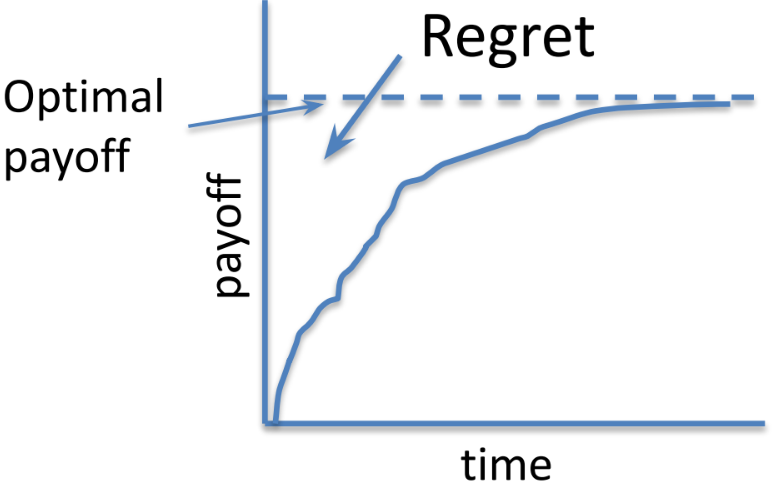
\includegraphics[width=0.6\linewidth]{resources/img/Regret_Optim_01.png}
    \caption{Regret}
    \label{fig:Regret}
\end{figure}

\subsection{PAC Optimality Frameworks}
\textbf{Probably Approximately Correct (PAC)} frameworks are usually used for identification of an $\epsilon$-optimal arm with probability $1-\delta$.

\noindent It is also $\epsilon$-optimal, meaning that, it satisfies the Mean of the selected arm.

\noindent Minimizes the Sample Complexity, i.e. the order of samples required for such an arm identification.

\section{Upper Confidence Bounds (UCB)}

\begin{minipage}{0.85\textwidth}
\begin{itemize}[leftmargin=*]
    \item Here, the arm with the best estimate $r^*$ so far serves as a benchmark, and other arms are played only if the upper bound of a suitable confidence interval is at least $r^*$.
    \item Simplest Approach --- Be Greedy with respect to UCBs.
    \item The Sub-optimal arm $j$ (say) is played fewer than $((8/\Delta_j) \ln n)$ times. 
    \item Further improvements on the base UCB Algorithm, called \texttt{UCB1}, focused mostly on reducing the constants.
    \item \texttt{UCB1} algo states that:\\
    \textbf{Loop: Until Convergence}\\
        \hspace{20pt} --- Play machine $j$ that maximizes $$\bar{x_j} + \sqrt{\frac{2 \ln n}{n_j}},$$ where $\bar{x_j}$ is the average reward obtained from machine $j$, $n_j$ is the number of times machine $j$ has been played so far, and $n$ is the overall (or total) number of plays done so far (including all arms).
\end{itemize}
\end{minipage}%
\hfill
\begin{minipage}{0.15\textwidth}
    % \centering
    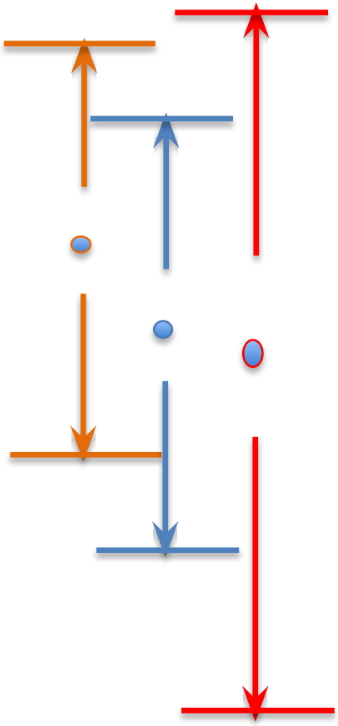
\includegraphics[width=\textwidth]{ucb_01.png}
\end{minipage}%


    
    \chapter{Features}

    \section{Mathematics}

    A few custom macros have also been added such as \texttt{\tbs{}rbk}, \texttt{\tbs{}sbk} and \texttt{\tbs{}cbk} for respectively round, square and curly brackets, \texttt{\tbs{}abs} for absulute value, \texttt{\tbs{}norm} for norm, \texttt{\tbs{}fact} for factorial and \texttt{\tbs{}diff} for up-right differential.
    $$
        \rbk{\frac{\pi}{2}}, \quad \sbk{\frac{\pi}{2}}, \quad \cbk{\frac{\pi}{2}}, \quad \abs{\frac{\pi}{2}}, \quad \norm{\frac{\pi}{2}}, \quad \fact{n} = \prod_{i = 1}^{n} i, \quad \frac{\diff \bm{x}}{\diff t} = \bm{v}
    $$

    Here are some examples showcasing what is possible with the default packages of \texttt{sleek}.

    \begin{equation}\label{eq:gauss_law}
        \oiint_S \bm{E} \cdot \diff \bm{s} = \iiint_V \frac{\rho}{\varepsilon_0} \diff V
    \end{equation}

    \begin{equation*}
        e = \sum_{n=0}^\infty \frac{1}{n!}
    \end{equation*}

    \begin{subequations}
        \begin{align}
            \frac{\diff x}{\diff t} & = \alpha x - \beta xy \\
            \frac{\diff y}{\diff t} & = \delta xy - \gamma y
        \end{align}
    \end{subequations}

    \begin{align*}
        \ln \abs{x} + C & = \int \frac{1}{x} \,\diff x \\
        \exp(x) & = \lim_{n \to \infty} \rbk{1 + \frac{x}{n}}^n
    \end{align*}

    \begin{equation}
        \left\{
        \begin{aligned}
            x & = r \sin \theta \cos \phi \\
            y & = r \sin \theta \sin \phi \\
            z & = r \cos \theta
        \end{aligned}
        \right.
    \end{equation}

    \begin{alignat*}{2}
                              & & P(A, B)  & = P(A \mid B) P(B)                        \\
        \Leftrightarrow \quad & & P(A \mid B) & = \frac{P(A, B)}{P(B)}                 \\
                              & &          & = P(B \mid A) \frac{P(A)}{P(B)}
    \end{alignat*}

    \subsection{Units}

    The \texttt{siunitx} package provides three commands to typeset numbers and quantities -- \texttt{\tbs{}num}, \texttt{\tbs{}si} and \texttt{\tbs{}SI} -- as well as various units (\emph{cf.} Table \ref{tab:siunitx_units}).

    It is possible to write, both in text or math modes, numbers without units (\emph{e.g.} \num{1}, \num{1.0}, \num{-1}, \num{3.14159}, \num{e100}, $N_A = \num{6.022e23}$), units without quantity (\emph{e.g.} $\si{\joule} = \si{\newton\meter} = \si{\kilogram\meter\squared\per\second\squared}$) and, finally, quantities with their units (\emph{e.g.} \SI{9.81}{\meter\per\second\squared}, $c = \SI{299.6e6}{\meter\per\second}$).

    \subsection{Lists}

    Sleek Template uses \texttt{enumitem} to enhance the listing capabilities of \LaTeX{}. There are three lists environments :
    \begin{enumerate}
        \item \texttt{itemize} for unordered lists;
        \item \texttt{enumerate} for ordered lists;
        \item \texttt{description} for descriptive lists.
    \end{enumerate}

    In a list, each element is preceded by the command \texttt{\tbs{}item}. It is possible to modify the labels
    \begin{itemize}
        \item individually with \texttt{\tbs{}item[newLabel]};
        \item for the whole environment with the \texttt{label=newLabel} option.
    \end{itemize}

    In the case of \texttt{enumerate}, \texttt{newLabel} can contain special expressions (\emph{cf.} Table \ref{tab:enumerate_special_expressions}) that will adapt to the item number. For example, \texttt{label=(\tbs{}alph*)} defines the label sequence \enquote{(a), (b), (c), ...}. Still in the case of \texttt{enumerate}, the  \texttt{\tbs{}setcounter} and \texttt{\tbs{}addtocounter} commands allow to modify the current item number.

    One could want to reduce the space between items with the \texttt{noitemsep} option or to delete the left margin with the \texttt{leftmargin=*} option.

    It is also possible to write nested lists. Here follows a very condensed example.

    \begin{itemize}[leftmargin=*]
        \item Lorem ipsum dolor sit amet, consectetur adipiscing elit, sed do eiusmod tempor incididunt ut labore et dolore magna aliqua.

        Arcu ac tortor dignissim convallis aenean et tortor. In eu mi bibendum neque egestas congue quisque.

        \item[$+$] Semper quis lectus nulla at volutpat diam ut. Felis eget velit aliquet sagittis id. Blandit aliquam etiam erat velit scelerisque in dictum non consectetur.
        \begin{equation}
            a^2 + b^2 = c^2
        \end{equation}

        \item Nibh sed pulvinar proin gravida hendrerit lectus. Pretium aenean pharetra magna ac placerat vestibulum lectus mauris. Non consectetur a erat nam at lectus urna duis.
        \begin{enumerate}[noitemsep, label=\roman*.]
            \item Nibh tortor id aliquet lectus. Sit amet justo donec enim diam vulputate ut pharetra sit.
            \setcounter{enumi}{3}
            \item Condimentum id venenatis a condimentum vitae. Quis eleifend quam adipiscing vitae proin sagittis nisl.
            \addtocounter{enumi}{15}
            \item Proin sagittis nisl rhoncus mattis rhoncus urna neque viverra.
        \end{enumerate}

        \item Elit scelerisque mauris pellentesque pulvinar pellentesque habitant morbi tristique senectus.
            \begin{description}
                \item[Ridiculus] mus mauris vitae ultricies leo. Mollis aliquam ut porttitor leo a diam. Velit egestas dui id ornare arcu odio ut sem nulla.
                \item[Nullam vehicula] ipsum a arcu. Nibh sit amet commodo nulla facilisi nullam. At erat pellentesque adipiscing commodo elit. Libero volutpat sed cras ornare arcu dui.
            \end{description}
    \end{itemize}

    \subsection{Tables}

    The packages \texttt{multicol} and \texttt{multirow} comes handy for complex table formatting such as multi-column or multi-row cells.

    \begin{table}[H]
        \centering
        \begin{tabular}{|r|r|c|l|}
            \hline
            \multicolumn{3}{|l|}{a} & qrs  \\ \hline
             b &  ef &     jkl      & tuvx \\ \hline
            cd & ghi &     mnop     & wyz  \\ \hline
        \end{tabular}
        \caption{Example of multi-column cells.}
        \label{tab:multicol_example}
    \end{table}

    \begin{table}[H]
        \centering
        \begin{tabular}{|l|c|r|}
            \hline
            \multirow{3}{2cm}{a} &   b   &    c \\ \cline{2-3}
                                 &  de   &   fg \\ \cline{2-3}
                                 &  hij  &  klm \\ \hline
            nopq                 & rstuv & wxyz \\ \hline
        \end{tabular}
        \caption{Example of multi-row cells.}
        \label{tab:multirow_example}
    \end{table}

    \newpage

    \section{\texttt{sleek-theorems}}

    \texttt{sleek-theorems} is based on the \texttt{amsthm} and \texttt{thmtools} packages. It provides a handful of theorem-like environments, each of which have different style and purpose.

    The environments are \texttt{thm} (theorem), \texttt{lem} (lemma), \texttt{prop} (proposition), \texttt{proof}, \texttt{defn} (definition), \texttt{hyp} (hypothesis), \texttt{meth} (method), \texttt{quest} (question), \texttt{answ} (answer), \texttt{expl} (example), \texttt{rmk} (remark), \texttt{note} and \texttt{tip}.

    \begin{note}
        The option \texttt{french} translates the name of each provided environment. It is also possible, and easy, to add your own language as an option in the source code.
    \end{note}

    \begin{thm}[Triangle inequality]
        Let be a triangle in Euclidean space. Then the sum of the lengths of two of its sides always surpass or equals the length of the third.
    \end{thm}

    \begin{proof}
        Let $a$, $b$ and $c$ be the lengths of the sides of a triangle in Euclidean space and $\alpha$, $\beta$, $\gamma$ their respective opposite angle. By the generalized Pythagoras' theorem, we have
        \begin{alignat*}{2}
                                  &  & c^2 & = a^2 + b^2 - 2ab \cos\gamma \\
                                  &  &     & \leq a^2 + b^2 + 2ab         \\
                                  &  &     & \leq (a + b)^2               \\
            \Leftrightarrow \quad &  & c   & \leq a + b
        \end{alignat*}
        Therefore in any triangle, the sum of the lengths of two sides always surpass or equals the length of the third.
    \end{proof}

    In addition, these environments also have framed versions -- \texttt{framedthm}, \texttt{framedlem}, etc. -- for readability.

    \begin{framedthm}[Triangle inequality]\label{thm:Triangle inequality}
        Let be a triangle in Euclidean space. Then the sum of the lengths of two of its sides always surpass or equals the length of the third.
    \end{framedthm}

    \begin{framedprf}
        Let $a$, $b$ and $c$ be the lengths of the sides of a triangle in Euclidean space and $\alpha$, $\beta$, $\gamma$ their respective opposite angle. By the generalized Pythagoras' theorem, we have
        \begin{alignat*}{2}
                                  &  & c^2 & = a^2 + b^2 - 2ab \cos\gamma \\
                                  &  &     & \leq a^2 + b^2 + 2ab         \\
                                  &  &     & \leq (a + b)^2               \\
            \Leftrightarrow \quad &  & c   & \leq a + b
        \end{alignat*}
        Therefore in any triangle, the sum of the lengths of two sides always surpass or equals the length of the third. \qedadd
    \end{framedprf}

    \begin{framedquest*}
        Based on the theorem \ref{thm:Triangle inequality}, what is the shortest path from a point $A$ to a point $B$ in Euclidean geometry ?
    \end{framedquest*}

    \newpage


    \printbibliography

    \appendix

    \chapter{Tables}

    \begin{table}[h]
        \centering
        \begin{tabular}{ll}
            \toprule
            \textbf{Package} & \textbf{Purpose} \\
            \midrule
            \texttt{amsmath} & Mathematical typesetting \\
            \texttt{amsthm} & Mathematical environments for theorems, proofs, etc. \\
            \texttt{booktabs} & Weighted rules for tables \\
            \texttt{biblatex} & Bibliography \\
            \texttt{csquotes} & Inline and display quotations \\
            \texttt{enumitem} & Lists and enumerations \\
            \texttt{float} & Floating objects such as figures and tables \\
            \texttt{graphicx} & Graphics \\
            \texttt{hyperref} & Hyperlinks and bookmarks \\
            \texttt{listings} & Code listings \\
            \texttt{multicol} & Table cells that span multiple columns \\
            \texttt{multirow} & Table cells that span multiple rows \\
            \texttt{siunitx} & Typesetting of units  \\
            \texttt{subcaption} & Sub-figures and sub-captions \\
            \bottomrule
        \end{tabular}
        \caption{List of the most relevant packages imported by Sleek Template.}
        \label{tab:sleek_relevant_packages}
    \end{table}

    \begin{table}[h]
        \centering
        \begin{tabular}{>{\ttfamily\tbs{}}ll}
            \toprule
            emph\{abcABC123\} & \emph{abcABC123} \\
            bfseries\{abcABC123\} & \bfseries{abcABC123} \\
            itshape\{abcABC123\} & \itshape{abcABC123} \\
            lowercase\{abcABC123\} & \lowercase{abcABC123} \\
            normalfont\{abcABC123\} & \normalfont{abcABC123} \\
            textbf\{abcABC123\} & \textbf{abcABC123} \\
            textit\{abcABC123\} & \textit{abcABC123} \\
            textsc\{abcABC123\} & \textsc{abcABC123} \\
            textsf\{abcABC123\} & \textsf{abcABC123} \\
            textsl\{abcABC123\} & \textsl{abcABC123} \\
            textsubscript\{abcABC123\} & \textsubscript{abcABC123} \\
            textsuperscript\{abcABC123\} & \textsuperscript{abcABC123} \\
            texttt\{abcABC123\} & \texttt{abcABC123} \\
            underline\{abcABC123\} & \underline{abcABC123} \\
            uppercase\{abcABC123\} & \uppercase{abcABC123} \\
            \bottomrule
        \end{tabular}
        \caption{Available text fonts in \LaTeX{}.}
        \label{tab:text_fonts}
    \end{table}

    \begin{table}[h]
        \centering
        \begin{tabular}{>{\ttfamily\$\tbs{}}l<{\$}l}
            \toprule
            mathcal\{abcABC123\} & $\mathcal{abcABC123}$ \\
            mathit\{abcABC123\} & $\mathit{abcABC123}$ \\
            mathnormal\{abcABC123\} & $\mathnormal{abcABC123}$ \\
            mathrm\{abcABC123\} & $\mathrm{abcABC123}$ \\
            mathbb\{abcABC123\} & $\mathbb{abcABC123}$ \\
            mathfrak\{abcABC123\} & $\mathfrak{abcABC123}$ \\
            \bottomrule
        \end{tabular}
        \caption{Available math fonts in \LaTeX{} and AMS.}
        \label{tab:math_fonts}
    \end{table}

    \begin{table}[h]
        \centering
        \begin{tabular}{>{\ttfamily}lr|>{\ttfamily}lr|>{\ttfamily}lr}
            \toprule
            metre & \si{\metre} & second & \si{\second} & mole & \si{\mole} \\
            meter & \si{\meter} & ampere & \si{\ampere} & candela & \si{\candela} \\
            kilogram & \si{\kilogram} & kelvin & \si{\kelvin} &  &  \\
            \midrule
            hertz & \si{\hertz} & farad & \si{\farad} & lumen & \si{\lumen} \\
            newton & \si{\newton} & ohm & \si{\ohm} & lux & \si{\lux} \\
            pascal & \si{\pascal} & siemens & \si{\siemens} & becquerel & \si{\becquerel} \\
            joule & \si{\joule} & weber & \si{\weber} & gray & \si{\gray} \\
            watt & \si{\watt} & tesla & \si{\tesla} & sievert & \si{\sievert} \\
            coulomb & \si{\coulomb} & henry & \si{\henry} &  &  \\
            volt & \si{\volt} & celsius & \si{\celsius} &  &  \\
            \midrule
            angstrom & \si{\angstrom} & day & \si{\day} & liter & \si{\liter} \\
            arcminute & \si{\arcminute} & degree & \si{\degree} & litre & \si{\litre} \\
            arcsecond & \si{\arcsecond} & electronvolt & \si{\electronvolt} & minute & \si{\minute} \\
            barn & \si{\barn} & gram & \si{\gram} & neper & \si{\neper} \\
            bar & \si{\bar} & hectare & \si{\hectare} & tonne & \si{\tonne} \\
            bel & \si{\bel} & hour & \si{\hour} &  &  \\
            \midrule
            yocto & \si{\yocto} & milli & \si{\milli} & mega & \si{\mega} \\
            zepto & \si{\zepto} & centi & \si{\centi} & giga & \si{\giga} \\
            atto & \si{\atto} & deci & \si{\deci} & tera & \si{\tera} \\
            femto & \si{\femto} & deca & \si{\deca} & peta & \si{\peta} \\
            pico & \si{\pico} & deka & \si{\deka} & exa & \si{\exa} \\
            nano & \si{\nano} & hecto & \si{\hecto} & zetta & \si{\zetta} \\
            micro & \si{\micro} & kilo & \si{\kilo} & yotta & \si{\yotta} \\
            \bottomrule
        \end{tabular}
        \caption{Available units in the \texttt{siunitx} package.}
        \label{tab:siunitx_units}
    \end{table}

    \begin{table}[h]
        \centering
        \begin{tabular}{ll}
            \toprule
            \textbf{Expression} & \textbf{Description} \\
            \midrule
            \texttt{\tbs{}arabic*} & Arabic numbers (1, 2, 3, ...) \\
            \texttt{\tbs{}alph*} & Lowercase letters (a, b, c, ...) \\
            \texttt{\tbs{}Alph*} & Uppercase letters (A, B, C, ...) \\
            \texttt{\tbs{}roman*} & Lowercase Roman numerals (i, ii, iii, ...) \\
            \texttt{\tbs{}Roman*} & Lowercase Roman numerals (I, II, III, ...) \\
            \bottomrule
        \end{tabular}
        \caption{Special expressions for the label of \texttt{enumerate} environments.}
        \label{tab:enumerate_special_expressions}
    \end{table}

\end{document}
